\documentclass[11pt,a4paper]{article}
\usepackage[utf8]{inputenc}
\usepackage[T1]{fontenc}
\usepackage{lmodern}
\usepackage[spanish,es-tabla]{babel}
\usepackage{graphicx} % Quita el [demo] para compilar con tus imágenes reales
\usepackage{geometry}
\usepackage[hidelinks]{hyperref}
\usepackage{float}
\usepackage{xcolor}
\usepackage{titlesec}
\usepackage{tcolorbox}
\usepackage{tabularx}
\usepackage{amssymb}
\usepackage{colortbl}
\usepackage{enumitem}

% Configuración de márgenes base
\geometry{top=2cm, bottom=2cm, left=1.8cm, right=1.8cm, columnsep=0.8cm}
\setlength{\parskip}{0.3em}

% Paleta de colores profesionales (Estilo DJI/Corporativo)
\definecolor{djidark}{RGB}{45,45,45}
\definecolor{djilight}{RGB}{120,120,120}
\definecolor{djiblue}{RGB}{0,112,192}

% Formateo de Títulos
\titleformat{\section}{\large\sffamily\bfseries\color{djidark}}{\thesection.}{0.5em}{}[\titlerule]
\titleformat{\subsection}{\normalsize\sffamily\bfseries\color{djidark}}{\thesubsection}{0.5em}{}

% Diseño de Cajas de Alerta y Notas
\tcbuselibrary{skins,breakable}
\newtcolorbox{warningbox}[1][]{
    enhanced,
    frame hidden,
    breakable,
    colback=gray!10,
    borderline west={3pt}{0pt}{red!80!black},
    fonttitle=\sffamily\bfseries\color{red!80!black},
    coltitle=red!80!black,
    title=ADVERTENCIA,
    attach title to upper=\quad,
    boxsep=2pt,
    left=4pt,
    right=4pt,
    top=4pt,
    bottom=4pt,
    #1
}

\newtcolorbox{infobox}[1][]{
    enhanced,
    frame hidden,
    breakable,
    colback=gray!5,
    borderline west={3pt}{0pt}{djiblue},
    fonttitle=\sffamily\bfseries\color{djiblue},
    coltitle=djiblue,
    title=NOTA,
    attach title to upper=\quad,
    boxsep=2pt,
    left=4pt,
    right=4pt,
    top=4pt,
    bottom=4pt,
    #1
}

\title{\vspace{-2cm}\sffamily\Huge\textbf{Manual de Operación y Ensamblaje}\\\vspace{0.5cm}\Large\color{djilight}{Plataforma Cuadricóptero - Controlador Cube}}
\author{\sffamily Victor Humberto Cruz Armijos \\ \textit{Escuela Politécnica Nacional}}
\date{\sffamily \today}

\begin{document}

% --- INICIO: SECCIÓN A UNA COLUMNA (PORTADA E ÍNDICE) ---
\maketitle

\begin{abstract}
El presente documento detalla el procedimiento técnico paso a paso como reporte final para la reconstrucción del chasis, configuración electrónica y de software de un vehículo aéreo no tripulado (cuadricóptero) utilizando un controlador de vuelo de la familia Cube (ej. Cube Black) con firmware ArduPilot, emisora Flysky FS-i6X y los softwares de estación terrena (QGroundControl y Mission Planner). Se documentan las observaciones descubiertas durante el ensamblaje, resolución de problemas de hardware, integración de módulos GNSS de precisión, telemetría avanzada, sintonización de PID en vuelo y protocolos operativos de seguridad civil para su despliegue en ecosistemas altoandinos.
\end{abstract}

\vspace{0.5cm}
\tableofcontents
\newpage

% --- INICIO: SECCIÓN A DOS COLUMNAS (CUERPO DEL MANUAL) ---
\twocolumn

\section*{Advertencias de Seguridad y Disclaimer}
\addcontentsline{toc}{section}{Advertencias de Seguridad y Disclaimer}

\begin{warningbox}[title=Precauciones Críticas de Seguridad Operativa]
La operación de Vehículos Aéreos No Tripulados (VANT) conlleva riesgos inherentes de carácter material y físico que el operador debe mitigar preventivamente.
\begin{itemize}[leftmargin=*,noitemsep]
    \item \textbf{Riesgo Eléctrico e Ignición:} Las baterías de Polímero de Litio (LiPo) son altamente volátiles. Se debe utilizar siempre bolsas ignífugas (\textit{LiPo Safe Bags}) para su transporte y proceso de carga.
    \item \textbf{Riesgo Mecánico (Hélices):} Las hélices rígidas girando a altas revoluciones pueden causar laceraciones graves. \textbf{Nunca} se debe armar el equipo ni conectar la batería principal en espacios cerrados sin retirar previamente las hélices.
    \item \textbf{Responsabilidad del Operador:} El ensamblador y piloto asumen total responsabilidad por daños a terceros. Cumplir con la normativa de la DGAC.
\end{itemize}
\end{warningbox}

\section{Lista de Componentes del Sistema y Ubicación Estratégica}
Hardware principal utilizado, priorizando el aislamiento electromagnético:
\begin{itemize}[leftmargin=*,noitemsep]
    \item \textbf{Controlador de Vuelo:} Autopiloto Cube Black integrado en su placa portadora (Carrier Board estándar).
    \item \textbf{Motores:} Motores Brushless (HobbyPower / equivalentes a AIR 2213 de 1000KV). 
    \item \textbf{Sistema de Radiocontrol:} Emisora Flysky FS-i6X sincronizada con un receptor FS-iA10B (protocolo i-BUS).
    \item \textbf{Sistema de Navegación:} Módulo Here GNSS, que incluye receptor de satélites y magnetómetro externo vía I2C.
    \item \textbf{Telemetría de Largo Alcance:} Módulos de radiofrecuencia operando en 433/915 MHz.
    \item \textbf{Fuente de Alimentación:} Batería LiPo de 3 celdas (3S).
    \item \textbf{Actuadores Adicionales:} Variadores de Velocidad (ESC) de 20A y hélices de plástico con rotación CW y CCW.
    \item \textbf{Estructura:} Chasis central en configuración cuádruple, tubos de fibra de carbono (10 mm) y acoples de unión (PETG/ABS).
\end{itemize}

\section{Observaciones de Ensamblaje: Precauciones de Hardware}

\subsection{Tornillería en Motores y Cortocircuitos}
Al fijar los motores brushless a la estructura o a los acoples impresos en 3D, la selección de la longitud de los tornillos es un factor de seguridad vital.

\begin{warningbox}[title=El Problema de los Cortocircuitos]
Un tornillo excesivamente largo penetrará la base del estator y perforará el esmalte aislante protector de las bobinas de cobre internas. Esto provoca un cortocircuito directo que viaja a través de la fibra de carbono (material conductivo), causando que el motor no gire, asimetrías de arranque o daños permanentes en los ESC. \textbf{Solución:} Siempre debe existir un espacio de separación (\textit{gap}) visible entre la punta del tornillo de sujeción y el bobinado.
\end{warningbox}

\section{Configuración del Enlace de Radio (Hardware)}

\subsection{Diferenciación de Enlaces}
Es fundamental separar físicamente el enlace de datos (telemetría) del enlace de radiocontrol.
\begin{itemize}[leftmargin=*,noitemsep]
    \item \textbf{Telemetría:} Transmite datos MAVLink a la estación terrena (433/915 MHz). Se conecta a los puertos \texttt{TELEM 1} o \texttt{TELEM 2}.
    \item \textbf{Radiocontrol:} Transmite los comandos de vuelo (2.4 GHz). Se conecta al puerto \texttt{RC IN} del Cube.
\end{itemize}

\subsection{Receptor Flysky FS-iA10B (i-BUS)}
Para evitar la latencia e interferencias del protocolo analógico PPM y omitir la inversión de S.BUS, se usa \textbf{i-BUS}:
\begin{enumerate}[leftmargin=*,noitemsep]
    \item \textbf{Selección de Puerto:} Utilizar \textbf{únicamente} el puerto horizontal superior etiquetado como \texttt{SERVO}.
    \item \textbf{Polaridad:}
    \begin{itemize}[noitemsep]
        \item \textbf{Señal (S):} Hacia el interior de la placa.
        \item \textbf{Voltaje (+):} Pin central (5V).
        \item \textbf{Tierra (-):} Hacia el borde exterior.
    \end{itemize}
    \item \textbf{Verificación de Energía:} El LED rojo debe encenderse de forma fija, indicando vinculación correcta.
\end{enumerate}

\subsection{Conexiones Centrales del Controlador}
El bloque central maneja la distribución de energía y las señales PWM hacia los variadores de velocidad.

\begin{figure}[H]
    \centering
    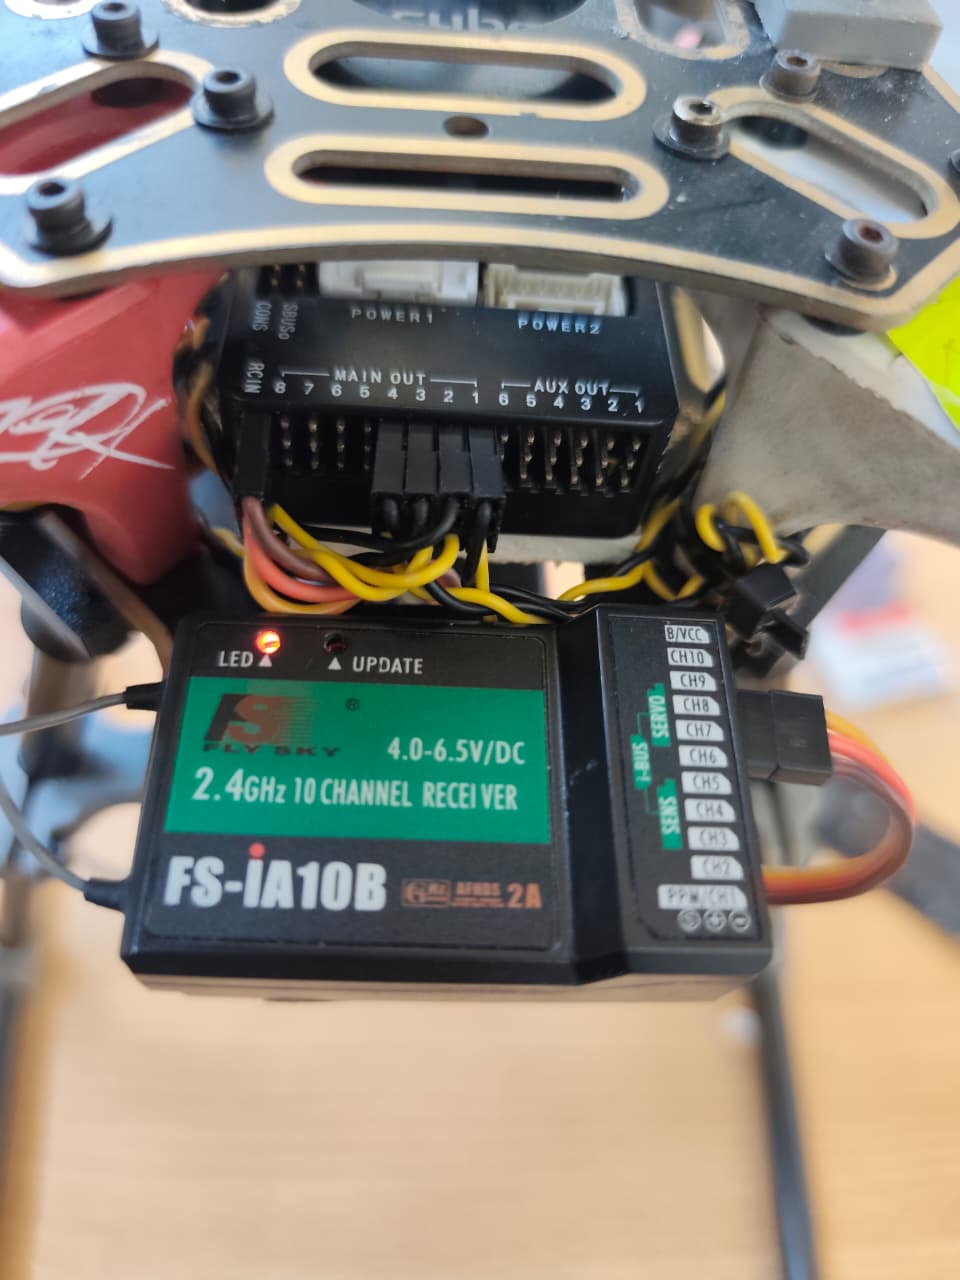
\includegraphics[width=0.45\textwidth]{CUBE_RECEPTOR.jpeg}
    \caption{Integración del controlador Cube y el receptor FS-iA10B. Conexión digital i-BUS en el puerto \texttt{SERVO}, alimentación por \texttt{POWER 1} y control de los ESC en \texttt{MAIN OUT}.}
\end{figure}

\section{Protocolo en la Emisora}
Para que la emisora envíe la información en formato digital sin inversiones lógicas por el puerto SERVO:
\begin{enumerate}[leftmargin=*,noitemsep]
    \item Mantener presionado el botón \texttt{OK} de la Flysky FS-i6X.
    \item Navegar a \texttt{System Setup} $\rightarrow$ \texttt{RX Setup} $\rightarrow$ \texttt{Output Mode}.
    \item Seleccionar la salida como \textbf{PWM \& i-BUS}. Evitar S.BUS.
    \item \textbf{Guardado:} Mantener presionado \texttt{CANCEL} durante 3 segundos.
\end{enumerate}

\section{Conexión al Software}
Para enlazar el controlador Cube a las estaciones terrenas:
\begin{itemize}[leftmargin=*,noitemsep]
    \item \textbf{Conexión alámbrica (USB):} Seleccionar el puerto COM correspondiente a \textbf{115200} baudios.
    \item \textbf{Conexión inalámbrica (Telemetría):} Al usar módulos RFD900, ajustar a \textbf{57600} baudios manualmente.
\end{itemize}

\section{Configuración Avanzada de Telemetría (RFD900)}
Para misiones autónomas o vuelos donde el dron excede la línea de visión directa (BVLOS), la estabilidad a 915 MHz es crítica.

\subsection{Emparejamiento y Ajuste de Potencia}
\begin{enumerate}[leftmargin=*,noitemsep]
    \item En Mission Planner, conectar vía USB al radio local (No al dron).
    \item Dirigirse a \texttt{Setup} $\rightarrow$ \texttt{Optional Hardware} $\rightarrow$ \texttt{SiK Radio} $\rightarrow$ \textbf{Load Settings}.
    \item \textbf{Net ID:} El parámetro crítico es el \textbf{Net ID}. Ambos radios deben poseer exactamente el mismo número (ej. \texttt{25}).
    \item \textbf{Regulación Termal:} Reducir \textbf{Tx Power} (medido en dBm) si las pruebas se realizan en laboratorio. Transmitir a 30 dBm (1 Vatio) en distancias cortas puede quemar el módulo. Para vuelos cortos, de 14 a 20 dBm es suficiente. Presionar \textit{Save Settings}.
\end{enumerate}

\begin{infobox}[title=Monitoreo del Enlace (RSSI)]
El RSSI debe revisarse en el HUD de Mission Planner. Valores cercanos a \textbf{200} indican una señal excelente. Si cae por debajo de \textbf{50-60} constantemente, existe riesgo inminente de desconexión (GCS Failsafe).
\end{infobox}

\section{Sincronización de ESC}
Para garantizar un despegue estable, los ESC deben memorizar los límites exactos de la señal de radio.

\subsection{Ajuste de Energía Base (Ralentí)}
En la pestaña \textit{Full Parameter Tree}:
\begin{itemize}[leftmargin=*,noitemsep]
    \item \textbf{MOT\_SPIN\_ARM:} \textbf{0.04} (4\%) Motores giran suave al armar.
    \item \textbf{MOT\_SPIN\_MIN:} \textbf{0.06} (6\%) Límite de seguridad en vuelo.
\end{itemize}

\subsection{Calibración Masiva (Vía Software)}
\begin{enumerate}[leftmargin=*,noitemsep]
    \item \textbf{Activación:} En Mission Planner, buscar \texttt{ESC\_CALIBRATION}, cambiar a \textbf{1} y \textit{Write Params}.
    \item \textbf{Reinicio:} Desconectar USB.
    \item \textbf{Aceleración Máxima:} Encender emisora y subir acelerador al \textbf{100\%}.
    \item \textbf{Energización:} Conectar LiPo (Forzar GPS \textit{Safety Switch} si existe).
    \item \textbf{Límite Inferior:} Tras escuchar \textbf{dos pitidos agudos}, bajar acelerador al \textbf{0\%}.
    \item \textbf{Guardado:} Los ESC emitirán un pitido largo. Desconectar batería.
\end{enumerate}

\subsection{Calibración Individual (CH3)}
Si la calibración masiva presenta asimetrías de encendido:
\begin{enumerate}[leftmargin=*,noitemsep]
    \item Desconectar cable PWM del ESC del Cube y conectarlo al \textbf{Canal 3 (CH3)} del receptor Flysky.
    \item Subir acelerador al \textbf{100\%} y conectar batería.
    \item Tras los \textbf{dos pitidos agudos}, bajar acelerador al \textbf{0\%}.
    \item Esperar el pitido largo y repetir por motor.
\end{enumerate}

\section{Integración Módulos GNSS (Here2)}
\subsection{Montaje Físico Estricto}
\begin{itemize}[leftmargin=*,noitemsep]
    \item \textbf{Orientación:} La flecha de la carcasa \textbf{debe apuntar exactamente} hacia el frente (nariz) del dron. Una desviación forzará un vuelo en espiral (efecto \textit{Toilet Bowl}).
    \item \textbf{Aislamiento:} Mástil alejado al menos 10 cm de la PDB y batería.
\end{itemize}

\subsection{Compensación Espacial (GPS Offset)}
Mida la distancia en metros desde el centro del Cube hasta el módulo GPS y configúrela en el \textit{Full Parameter Tree} (NED):

\begin{warningbox}[title=La Trampa del Eje Z (NED)]
ArduPilot utiliza el estándar aeroespacial NED (North, East, Down). Esto significa que el eje Z es \textbf{positivo hacia abajo}. Como el GPS va montado en un mástil por encima de la placa, el valor Z debe ser estrictamente \textbf{negativo} (ej. \texttt{-0.15}).
\end{warningbox}

\begin{itemize}[leftmargin=*,noitemsep]
    \item \textbf{GPS\_POS1\_X:} Distancia longitudinal.
    \item \textbf{GPS\_POS1\_Y:} Distancia lateral.
    \item \textbf{GPS\_POS1\_Z:} Altitud del mástil (\textbf{Negativo}).
\end{itemize}

\section{Calibración de Sensores Inerciales}
\begin{enumerate}[leftmargin=*,noitemsep]
    \item \textbf{Radio:} En \textit{Radio Calibration}, mover joysticks a sus límites mecánicos máximos. Guardar con \textbf{Done}.
    \item \textbf{Acelerómetro:} En \texttt{Setup}, seleccionar \texttt{Accelerometer} (\texttt{Rotation} en \textbf{None}) e inmóvil en las 6 orientaciones.
    \item \textbf{Compás:} Priorizar compás externo en \texttt{Compass}. Ejecutar \textit{Onboard Mag Calibration} girando el dron. Cambiar \texttt{COMPASS\_LEARN} a \textbf{3} (InFlight).
\end{enumerate}

\section{Prevención de Interferencias (EMI)}
\begin{itemize}[leftmargin=*,noitemsep]
    \item \textbf{Alejar PDB y Baterías:} Son los mayores generadores de ruido.
    \item \textbf{Trenzado de Cables:} Trenzar los cables de alta corriente (positivo y negativo) cancela los campos magnéticos opuestos.
\end{itemize}

\section{Análisis de Registros (DataFlash)}
\subsection{Consumo de Batería y Eficiencia}
En \textbf{BAT} $\rightarrow$ \textbf{0}:
\begin{itemize}[leftmargin=*,noitemsep]
    \item \textbf{Voltage Sag:} Comparar \texttt{Volt} vs \texttt{VoltR}. Una caída severa (mayor a 1.0V) al acelerar indica batería degradada.
    \item \textbf{Capacidad Consumida:} \texttt{CurrTot} suma los mAh extraídos. Si consume más del 80\% en menos de 10 min, optimice el MTOW.
\end{itemize}

\subsection{Salud de Vuelo}
\begin{itemize}[leftmargin=*,noitemsep]
    \item \textbf{EKF:} Graficar \textbf{SM} en \textbf{XKF4}. Debe mantenerse $< 0.5$.
    \item \textbf{Vibraciones:} \texttt{VibeX, VibeY, VibeZ} $< 30 m/s^2$. \texttt{Clip} estrictamente en \textbf{0}.
    \item \textbf{Motores:} \texttt{C1} a \texttt{C4} en \textbf{RCOU} deben agruparse uniformemente.
\end{itemize}

\section{Optimización de Control}
\subsection{Aprendizaje de Vuelo (Hover)}
\begin{enumerate}[leftmargin=*,noitemsep]
    \item \textbf{MOT\_HOVER\_LEARN} al valor \textbf{2}.
    \item Vuelo estacionario ininterrumpido en \textbf{Loiter} durante 30 segundos.
\end{enumerate}

\subsection{Filtro de Muesca Armónico}
Para cancelar algoritmicamente la resonancia:
\begin{enumerate}[leftmargin=*,noitemsep]
    \item \textbf{INS\_HNTCH\_ENABLE} = 1.
    \item \textbf{INS\_HNTCH\_MODE} = 1.
    \item \textbf{INS\_HNTCH\_REF} = Valor de \textbf{MOT\_THST\_HOVER}.
    \item \textbf{Registros FFT:} \textbf{INS\_LOG\_BAT\_MASK} = 1 y \textbf{INS\_LOG\_BAT\_OPT} = 2.
\end{enumerate}

\subsection{Sintonización Dinámica (Canal 6)}
\begin{enumerate}[leftmargin=*,noitemsep]
    \item \textbf{Emisora:} Asignar \textbf{Channel 6} a \textbf{VrA}.
    \item \textbf{Mission Planner:} En \texttt{Extended Tuning} (canal 6), seleccionar \textbf{Rate Roll/Pitch kP}. \textbf{Min: 0.080}, \textbf{Max: 0.200}.
    \item \textbf{Operación:} Perilla en la mitad ($\approx 0.14$). Si oscila rápido, girar izquierda (Min). Si se siente blando, girar derecha (Max).
\end{enumerate}

\section{Modos de Vuelo y Códigos LED}
\begin{itemize}[leftmargin=*,noitemsep]
    \item \textbf{Stabilize:} Control de actitud puro. Nivelación manual.
    \item \textbf{AltHold:} Mantenimiento automático de altura por Barómetro.
    \item \textbf{Loiter:} Barómetro + GPS mantienen posición en 3D.
    \item \textbf{Auto:} Vuelo autónomo por waypoints.
    \item \textbf{RTL:} Asciende, regresa a Home y aterriza.
\end{itemize}

\begin{infobox}[title=Diagnóstico LED del Cube]
\textbf{Verde Parpadeante:} GPS \textit{3D Fix} adquirido (Listo para armar). \textbf{Amarillo Parpadeante:} Falla en pruebas pre-armado. \textbf{Rojo Parpadeante:} \textit{Failsafe} activado.
\end{infobox}

\section{Protocolos de Seguridad (Failsafes)}
\begin{itemize}[leftmargin=*,noitemsep]
    \item \textbf{RC Failsafe:} RTL automático si se pierde radio.
    \item \textbf{Battery Failsafe:} \textit{Land} o \textit{RTL} a \textbf{10.5V} (3S).
    \item \textbf{Compensación de Voltaje:} Asignar \texttt{BATT\_FS\_VOLTSRC} a \textbf{1} para monitorear el voltaje compensado y evitar falsos positivos por picos de amperaje.
\end{itemize}

\section{Planificación Autónoma (Auto)}
\begin{enumerate}[leftmargin=*,noitemsep]
    \item Dibujar polígono en la pestaña \textbf{Plan}.
    \item Clic derecho $\rightarrow$ \textit{Auto WP} $\rightarrow$ \textit{Survey (Grid)}.
    \item Configurar \textit{Overlap} al \textbf{70\%} mínimo para fotogrametría.
    \item Clic en \textbf{Write} para enviar al Autopiloto.
\end{enumerate}

\section{Consideraciones a Gran Altitud}
En ecosistemas andinos (2,850 m.s.n.m.):
\begin{itemize}[leftmargin=*,noitemsep]
    \item \textbf{Baja Densidad del Aire:} Los motores girarán a mayores RPM para sostener el mismo peso.
    \item \textbf{Reducción de Autonomía:} El tiempo de vuelo se reduce un \textbf{15\% a 25\%}.
    \item \textbf{Refrigeración Ineficiente:} El riesgo de sobrecalentamiento en ESC y motores aumenta.
\end{itemize}

\section{Mantenimiento Post-Vuelo}
\begin{itemize}[leftmargin=*,noitemsep]
    \item \textbf{Baterías LiPo 1C:} Cargar a la regla de "1C" (Ej. 5200 mAh a 5.2A máximo). Almacenar en \textit{Storage} (\textbf{3.8V} por celda) si no se usa en 48 horas.
    \item \textbf{Rodamientos:} Sustituir al detectar sonido arenoso.
    \item \textbf{Fatiga Estructural:} Usar Locktite azul solo en uniones metal-metal. Reemplazar hélices ante la mínima fisura o línea de estrés.
\end{itemize}

\subsection{Guía de Choque (Crash Guide)}
Si el equipo sufre impacto: 1) Acérquese por detrás y \textbf{desconecte la batería LiPo inmediatamente} (previene incendio). 2) No apague la radio. 3) Extraiga la MicroSD.

% --- INICIO: SECCIÓN A UNA COLUMNA (ANEXOS Y CHECKLIST) ---
\onecolumn
\newpage
\section*{Lista de Chequeo Pre-Vuelo (Pre-Flight Checklist)}
\addcontentsline{toc}{section}{Lista de Chequeo Pre-Vuelo}
Ejecutar inspección mandatoria previo al armado de motores. \vspace{0.5cm}

\renewcommand{\arraystretch}{1.8}
\begin{table}[H]
    \centering
    \begin{tabularx}{\textwidth}{|p{1cm}|X|p{2cm}|}
    \hline
    \rowcolor{djidark}
    \multicolumn{3}{|c|}{\textcolor{white}{\textbf{\sffamily FASE 1: INSPECCIÓN MECÁNICA Y ESTRUCTURAL}}} \\ \hline
    $\square$ & \textbf{Hélices:} Fijadas sin holgura. Roscas en buen estado. & \quad OK \\ \hline
    $\square$ & \textbf{Rotación:} Hélices CW/CCW instaladas en los motores correctos. & \quad OK \\ \hline
    $\square$ & \textbf{Integridad Palas:} Sin fisuras, rasguños profundos o líneas blancas de estrés. & \quad OK \\ \hline
    $\square$ & \textbf{Motores:} Giro libre con la mano (sin resistencia de rodamientos o arena). & \quad OK \\ \hline
    $\square$ & \textbf{Chasis:} Tornillería de brazos y bancadas apretada. Estructura rígida. & \quad OK \\ \hline
    $\square$ & \textbf{GPS:} Mástil fijo. Flecha del módulo alineada exactamente a la nariz del dron. & \quad OK \\ \hline
    $\square$ & \textbf{Telemetría:} Antenas RFD900 aseguradas verticalmente, lejos de la fibra de carbono. & \quad OK \\ \hline
    $\square$ & \textbf{Carga Útil:} Gimbal / Cámara asegurada. Tarjeta de memoria insertada. & \quad OK \\ \hline

    \rowcolor{djidark}
    \multicolumn{3}{|c|}{\textcolor{white}{\textbf{\sffamily FASE 2: ENERGÍA Y ESTACIÓN TERRENA}}} \\ \hline
    $\square$ & \textbf{Batería (LiPo):} Voltaje $> 12.4V$ (3S al 100\%). Celdas balanceadas. & \quad OK \\ \hline
    $\square$ & \textbf{Fijación Batería:} Sujeta firmemente con velcro para evitar desplazamientos del CG. & \quad OK \\ \hline
    $\square$ & \textbf{Emisora Radio:} Encendida. Voltaje correcto. Palanca de acelerador abajo. & \quad OK \\ \hline
    $\square$ & \textbf{Interruptores:} Asignados a posición segura (Modo Loiter o Stabilize seleccionado). & \quad OK \\ \hline
    $\square$ & \textbf{Estación Terrena:} Mission Planner o QGC conectado. Telemetría sincronizada. & \quad OK \\ \hline

    \rowcolor{djidark}
    \multicolumn{3}{|c|}{\textcolor{white}{\textbf{\sffamily FASE 3: COMPROBACIONES DE SOFTWARE (HUD)}}} \\ \hline
    $\square$ & \textbf{Enlace Radio:} RSSI estable por encima de 80. Sin caídas súbitas. & \quad OK \\ \hline
    $\square$ & \textbf{Salud EKF:} Indicador EKF en color blanco o verde (Jamás rojo intermitente). & \quad OK \\ \hline
    $\square$ & \textbf{Navegación GNSS:} Señal \textit{3D Fix} confirmada. & \quad OK \\ \hline
    $\square$ & \textbf{Satélites:} Mínimo 12 satélites conectados (Preferible $>$ 15). & \quad OK \\ \hline
    $\square$ & \textbf{Precisión Geométrica:} HDOP inferior a 1.0 (Óptimo $<$ 0.8). & \quad OK \\ \hline
    $\square$ & \textbf{Horizonte Artificial:} Responde correctamente al mover físicamente el chasis. & \quad OK \\ \hline
    \end{tabularx}
\end{table}

\vspace{0.5cm}
\begin{infobox}[title=Protocolo Inaugural (Maiden Flight)]
En el primer despegue del día, armar y elevar el dron a \textbf{1.5 metros} en modo Loiter. Soltar las palancas (Hands-off) para confirmar que no existe derivación (Drift). Aterrizar a los 3 minutos para evaluar temperatura de los motores y ESC.
\end{infobox}

\newpage
\appendix
\section{Anexo A: Historial de Resolución de Problemas}
\subsection{Asimetría y Falsa Zona Muerta (28\%)}
Durante las pruebas de integración, el Autopiloto requería inyectar un 28\% de aceleración nominal para que los motores rompieran la estática. La calibración masiva (\texttt{ESC\_CALIBRATION}) generó arranques inseguros.

\textbf{Resolución:} Se aisló el hardware, conectando los ESC directamente al puerto \texttt{CH3} del receptor Flysky. Esta calibración hardware a hardware redujo la zona muerta, permitiendo regresar los parámetros \texttt{MOT\_SPIN\_ARM} (4\%) y \texttt{MOT\_SPIN\_MIN} (6\%) a niveles estandarizados.

\vspace{1cm} % Espacio entre anexo A y B para que no se peguen tanto pero se mantengan en la misma hoja
\section{Anexo B: Reseteo de Radio FS-i6X}
\subsection{Recuperación por Bloqueo de Calibración}
Si la calibración de radio falla o se bloquea:
\begin{enumerate}[leftmargin=*,noitemsep]
    \item \textbf{Reset de Software:} En \texttt{Full Parameter List}, seleccionar \textbf{Reset to Default} y reiniciar el Autopiloto.
    \item \textbf{Reset de Emisora:} En la Flysky, ir a \texttt{System Setup} $\rightarrow$ \texttt{Factory Reset}.
    \item Volver a vincular el receptor y configurar \textbf{Output Mode} a \textbf{i-BUS}.
\end{enumerate}

\subsection{Ejes Máximos (Endpoints)}
\begin{enumerate}[leftmargin=*,noitemsep]
    \item En la radio, ir a \texttt{Functions setup} $\rightarrow$ \texttt{Endpoints}. Los canales del 1 al 4 deben indicar \textbf{100\%} en ambos extremos.
    \item En \texttt{Aux. channels}, asignar el \textbf{Canal 5} a un interruptor de 3 posiciones (ej. \textbf{SwC}) para modos de vuelo.
    \item Asignar el \textbf{Canal 6} a una perilla giratoria (ej. \textbf{VrA}) para sintonización.
\end{enumerate}

\newpage
\section{Anexo C: Glosario de Términos Aeronáuticos}
\begin{itemize}[leftmargin=*]
    \item \textbf{BVLOS (Beyond Visual Line of Sight):} Operaciones aéreas donde el dron vuela más allá de la línea de visión directa del piloto.
    \item \textbf{EKF (Extended Kalman Filter):} Algoritmo matemático que fusiona los datos del GPS, barómetro, giroscopio y acelerómetro para predecir la posición y actitud del dron.
    \item \textbf{ESC (Electronic Speed Controller):} Variador de velocidad encargado de traducir las señales digitales de la controladora en pulsos trifásicos de potencia.
    \item \textbf{GNSS (Global Navigation Satellite System):} Término técnico general que engloba a todos los sistemas de posicionamiento por satélite (GPS, GLONASS, Galileo, BeiDou).
    \item \textbf{HDOP (Horizontal Dilution of Precision):} Medida geométrica que indica la precisión de la posición GPS. Valores por debajo de 1.0 garantizan un modo \textit{Loiter} sólido.
    \item \textbf{MTOW (Maximum Take-Off Weight):} Peso Máximo al Despegue. Es el límite físico que el dron puede levantar antes de sobrecalentarse.
    \item \textbf{PWM (Pulse Width Modulation):} Señal eléctrica estandarizada que utiliza el Autopiloto para enviar comandos de velocidad (usualmente entre 1000 y 2000 microsegundos).
    \item \textbf{RSSI (Received Signal Strength Indicator):} Métrica que cuantifica el nivel de potencia de la señal de radio recibida por las antenas.
\end{itemize}

\end{document}
